Android je mobilní operační systém vyvíjený společností Google, který je založený na Linuxovém jádře. Je vyvíjen jako opensource a používá se především v mobilních zařízeních jako jsou chytré telefony, hodinky a tablety. Můžeme jej však také nalézt také v přístrojích jako jsou set-top boxy, multimediální přehrávače a v jiné elektronice.\\
\section{Historie}
Počátky Androidu spadají do roku 2003, kdy byla v Kalifornii v USA založena společnost Android, Inc. O Dva roky později firmu odkupuje světoznámá společnost Google. V roce 2007 získává Google několik patentů v oblasti mobilních zařízení a 5. listopadu téhož roku dochází k oficiálnímu představení a vzniká sdružení firem Open Handset Alliance, která mé za cíl vytvoření otevřených standartů v oblasti mobilních zařízení. V tabulce TODO odkaz je zobrazena stručná historie verzí operačního systému Android.

\begin {table}[h!]
\begin{tabular}{|l|c|l|c|}
\hline
{\bf Datum}         & {\bf Verze}   & {\bf Označení}        & {\bf Verze API}   \\
\hline \hline
23. září 2008       & 1.0 -- 1.1    & --                    & 1 -- 2            \\
\hline
April 27, 2009      & 1.5           & Cupcake               & 3                 \\
\hline
September 15, 2009  & 1.6           & Donut                 & 4                 \\
\hline
October 26, 2009    & 2.0 -- 2.1    & Eclair                & 5 -- 7            \\
\hline
May 20, 2010        & 2.2 -- 2.2.3  & Froyo                 & 8                 \\
\hline
December 6, 2010    & 2.3 -- 2.3.7  & Gingerbread           & 9 -- 10           \\
\hline
February 22, 2011   & 3.0 -- 3.2    & Honeycomb             & 11 -- 13          \\
\hline
October 18, 2011    & 4.0 -- 4.0.4  & Ice Cream Sandwich    & 14 -- 15          \\
\hline
July 9, 2012        & 4.1 -- 4.3    & Jelly Bean            & 16 -- 18          \\
\hline
October 31, 2013    & 4.4           & KitKat                & 19 -- 20          \\
\hline
November 12, 2014   & 5.0           & Lollipop              & 21                \\
\hline
\end{tabular}
\centering
\caption{Verze operačního systému Android}
\end{table}

\section{Arcitektura}
Architektura systému android je složena z šesti vrstev:
\begin{itemize}
\item Linuxové jádro
\item HAL
\item Knihovny
\item Android runtime
\item Application framework
\item Aplikace
\end{itemize}

\begin{figure}[h!]
    \centering
    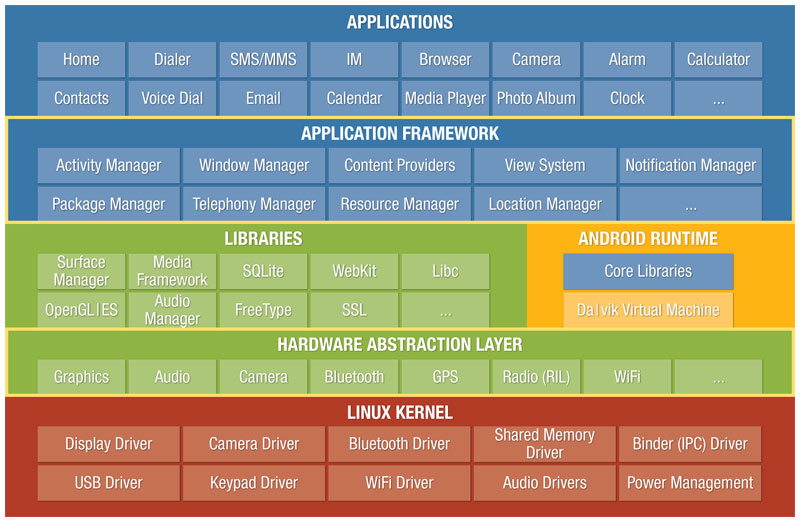
\includegraphics[scale=0.5]{fig/android_architecture.jpg}
    \caption{Android architecture}
\end{figure}

\subsection{Linuxové jádro} %https://source.android.com/devices/
Tato nejnižší vrstva je postavena mezi hardware zařízení a ostatní vrstvy architektury. Android je postavený na zvlaštní verzi Linuxového jádra a několika speciálními doplňky jako jsou správa systémové paměti, the Binder IPC driver, and other. Od počátku byl android postaven na linuxovém jádru 2.6, nejnověší android pak běží na jádru 3.4.  Při startu se jádro zavede do operační paměti a je mu předáno řízení.
\subsection{Hardware abstraction layer (HAL)} %https://source.android.com/devices/
HAL je standartní rozhraní které umožňuje systému android volat do vrstvy ovladačů, zatímco je mu jedno jaká je implementace v nižších vrstvách obladačů a hardwareru. Pro každý kus hardwaru by měl existovat ovladač a k němu odpovídající HAL poskytující možnosti hardwaru.
\subsection{Knihovny}
Nad HAL vrstvu se nachází vrstva nativních knihoven. Tyto knihovny jsou napsány v jazyce C nebo C++. K těmto knihonám se dá přistoupit přes android sdk pokud je však požadován přímý přístup je možné to provést přes NDK. Mezi tyto knihovny patří:
\begin{itemize} %http://www.android-app-market.com/android-architecture.html
\item Surface manager -- knihovna pro skládání oken na obrazovce
\item Media Framework -- poskytuje různé multimediální kodeky pro nahrávání a přehrávání videa v různých formátech.
\item SQLite -- databázový engine pro použítí v oblasti uložení dat
\item WebKit -- prohlížečový enginepro  zobrazování webového obsahu
\item Libc -- standartní knihovna jazyka C 
\item OpenGL ES -- knihovna pro podporu 2D a 3D grafiky a renderování.
\item Audio Manager -- knihovna pro práci se zvuky zařízení
\item FreeType -- knihovna pro bitmapové a vektorové vykreslení písma
\item SSL -- knihovna pro využití šifrovacího protokolu pro bezpečnou intenetovou komunikaci.
\item and others.
\end{itemize}


\subsection{Android runtime}
Vedle vrstvy nativních knihoven se nachází se nachází Android Runtime vrstva, která se skládá ze dvou základních částí a to z Core Libraies a z Dalvik Virtual Machine (DVM). Core libraries jinak řečené Android API pak můžeme rozdělit ještě na dvě částí a to Java Knihovny a Android knihovny.

\subsubsection{Dalvik Virtual Machine (DVM)}
DVM je virtuální stroj, který je vyvíjen od roku 2005 a byl do systému uzačleněn z důvodu, že JVM není licencován jako opensource a druhým důvodem byla optimalizace pro mobilní zařízení.

Každá aplikace beží na android zařízení v rámcí své vlastníá instance DVM, tedy nikoliv jako proces přímo v linuxovém jádře.

Spouštění aplikací na Virtuálních strojích přináší řadu výhod.  Jednak se jedná o to že pracují v izolovaném prostoru a tudíž nemohou zasáhnout do operačního systému či do jiných aplikací. Za druhé to činí z aplikace platformně nezávislou a tak může být zpuštěnan na jakémkoliv hardwaru.

Mezi výhody DVM patří jeho efektivnost ve využívání paměti a díky tomu je lépe přizpůsoben k použití na mobilních zařízeních.

Proto aby mohla být aplikace spuštěna v DVM, kód aplikace musí být transformován ze standartních java souboru do dalvik executables (.dex format). K tomuto se používá dx nástroj ktérý tento převod vykonává.
\subsubsection{Java knihovny}
Většina Android aplikací je napsána pomocí jazyka Java. Tyto Java knihovny jsou opensource implementaci knihoven založenou na Apache Harmony Projektu a jedná se o podmnožinu Java SE platformy. Neobsahují např. knihovny java.awt nebo java.swing, které jsou nahrazeny vlastními třídami pro tvorbu uživatelského rozhrani Android aplikací. Podrobnější srovnání je možné nalezt v kapitole TODO. 
\subsubsection{Android knihovny}
Jedná se o specifické knihovny, které poskytují veškerou funkcionalitu android zařízení. Knihovny jsou napsány v jazyku Java a patří mezi ně tyto balíky:
\begin{itemize}
\item android.app -- poskytuje přístup k aplikačnímu modelu a je základním kamenem všech aplikací 
\item android.content -- obsahují třídy pro přístup a publikování dat aplikací
\item android.database -- třídy pro přístup k datům a manipulaci s databazemi
\item android.graphics -- knihovny pro vykreslování na obrazovku
\item android.hardware -- poskytují přístup k hardware funkcím jako jsou kamera a sensory
\item android.media -- knihovny pro práci s ultimédii
\item android.text -- knihovny pro praci s řetězci a ajejich zobrazením na display
\item android.util -- bežné nástroje jako manipulace s daty a časem převody mezi čísly a řetězci a další 
\item android.view -- základní stavební blok pro budování grafického uživatelského rozhraní
\item android.webkit -- knihovny pro práci s webovým obsahem
\item and others.
\end{itemize}

\subsection{Application framework}
Vrstva aplikačního frameworku poskytuje mnoho vysoko-úrovňových služeb aplikacím ve formě java knihoven. Pro vývojáře se jedná o nejdůležitější vrstvu,která umožňuje přístup ke službám daného zařízení. Tato vrstva je tvořena: 
\begin{itemize} %http://developer.android.com/reference/
\item Activity manager -- ovládání životního cyklu aplikací jejich start průběh a konec
\item Windows manager -- pro správu viditelnosti oken a jejich uspořádání
\item Content Providers -- umožňuje pracovat s obsahem jiných aplikací, poskytuje mechanismy pro jejich zabezpečení 
\item View System -- View je základní stavební blok pro komponenty uživatelského rozhraní. View systém je sada View která slouží k budování uživatelského rozhraní aplikace.
\item Notification manager -- Umožňuje uživatele informovat pomocí alertů a notifikací.
\item Package manager -- Umožňuje získat různé informace o aplikacích které jsou aktuálně naisntalovány  zařízení.
\item Telephony manager -- Poskytuje přístup k telefoním službám zařízení. 
\item Resource manager -- Umožňuje přístup ke zdrojům jako jsou barevná nastavení, rozvržení a stringy.
\item Location manager - Poskytuje přístup k systémovým lokačním službám. Tyto služby umožňují v pravidelných intervalech získávat geografick souřadnice zařízení.
\item and others.
\end{itemize}

\subsection{Aplikace}
Poslední a nejvyšší vrstva se skládá ze samotných aplíkací. Jendak se jedná o předinstalované aplikace a druhak se jedná o aplikace, které byly postupem času přidány z android obchodu nebo jinou cestou.




\section{Struktura aplikace}
\subsection{Prvky}
\subsubsection{Aktivity}
\subsubsection{Služby}
\subsubsection{Content providers}
\subsubsection{Intents}
\subsubsection{Broadcast receivers}
\subsubsection{Notification}

\subsection{Application Resources}
\subsection{Application Manifest} % http://developer.android.com/guide/topics/manifest/manifest-intro.html
Každá aplikace ve své rootovské složcě musí mít soubor AndroidManifest.xml. Tento soubor obsahuje informace o aplikaci s ohledem na systém Android. 
\subsection{User Interface}

\section{Android SDK}
?????? TODO .. nevim jestli je potřeba
\section{Build System}%http://developer.android.com/sdk/installing/studio-build.html
Build System je způsob jakým se vyprodukuje ze zdrojového kódu a závislostí a reourců .apk balík. Celý tento proces je automatizován pomocí gradle skriptů ale je pro portování aplikací je dobré mu porozumět.

\subsection{Build Process}
Ná obrázku je možné vidět jakým způsobem probíhá vytváření .apk balíčku. Jednotlivé kroky jsou pak tyto:
\begin{enumerate}
\item The Android Asset Packaging Tool zkompiluje resource soubory jako jsou manifest a xml soubory a vyprodukuje R.java takže je možné se na resourcy odkazovat.
\item Aidl konvertuje všechny .aidl rozhraní do java rozhraní
\item Všechen kód je zkompilován java kompilátorem, výstupem jsou .class soubory.
\item Nástroj dex převede .class soubory do Dalvik byte kodu. Stejně tak soubory třetích stran
\item Všechny nokompilované resourcy (např. obrázky), kompilované resourcy a .dex soubory jsou poslany apkbuilderu aby je zabalil do .apk souboru.
\item Poté musím byt .apk podepsán.
\item Nakonec pokud je podepsán v release módu musí být zipalign nástrojem vyrovnán a tím se sníží paměťová náročnost.
\end{enumerate}

\begin{figure}[h!]
    \centering
    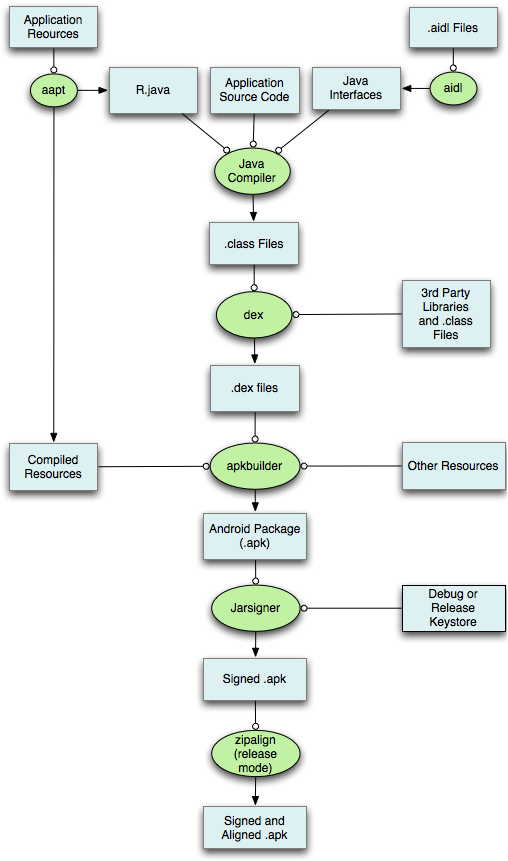
\includegraphics[scale=0.6]{fig/build.png}
    \caption{Build process}
\end{figure}



